\section{Horizon Transfer Analysis}
\label{app:horizon}

\cref{tab:horizon} shows the $\Delta{=}1$ vs.\ $\Delta{=}3$ comparison.
At $\Delta{=}1$, SGTONetV6 substantially outperforms all baselines on class-9 F1.
At $\Delta{=}3$, PatchTST achieves macro-F1 0.588 and class-9 F1 0.192, while SGTONetV6 achieves macro-F1 0.501 and class-9 F1 0.107.
The rare trigger still improves recall at $\Delta{=}3$ but loses precision, so false positives dominate.
The formal claim of this paper is therefore restricted to the short-horizon $\Delta{=}1$ setting.

\begin{table}[h]
\centering
\caption{Horizon transfer: $\Delta{=}1$ vs.\ $\Delta{=}3$. SGTONetV6 is strongest at $\Delta{=}1$; PatchTST outperforms at $\Delta{=}3$.}
\label{tab:horizon}
\begin{tabular}{llrrr}
\toprule
$\Delta$ & Method & Macro-F1 & Bal.\ Acc. & Cls-9 F1 \\
\midrule
1 & \textbf{SGTONetV6} & \textbf{62.3} & \textbf{67.3} & \textbf{55.6} \\
1 & PatchTST & 56.9 & 61.5 & 0.0 \\
\midrule
3 & PatchTST & \textbf{58.8} & \textbf{63.1} & \textbf{19.2} \\
3 & SGTONetV6 & 50.1 & 61.1 & 10.7 \\
3 & SGTONetV4 & 48.1 & 54.7 & 0.0 \\
\bottomrule
\end{tabular}
\end{table}

\begin{figure}[h]
  \centering
  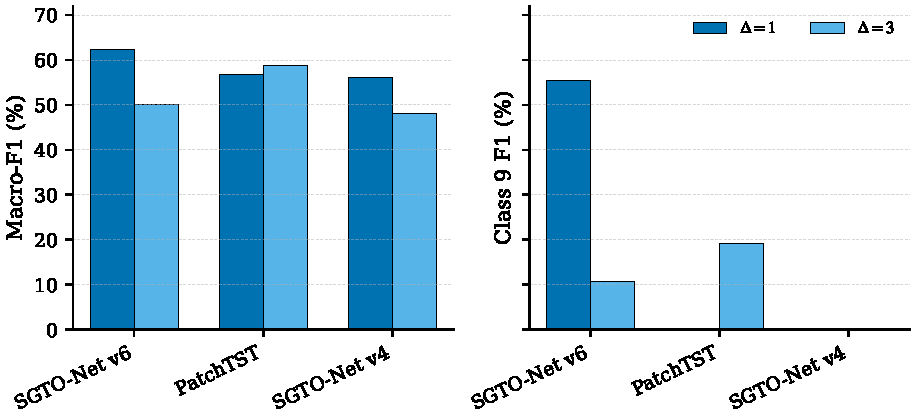
\includegraphics[width=0.95\linewidth]{figures/fig4_horizon_transfer.pdf}
  \caption{Horizon comparison. SGTONetV6 is strongest for short-horizon $\Delta{=}1$ rare-fault recovery and does not transfer directly to $\Delta{=}3$.}
  \label{fig:horizon}
\end{figure}

\section{Threshold Sensitivity}
\label{app:threshold}

\cref{fig:threshold} shows the rare-trigger threshold sensitivity curve.
The best tested global threshold is approximately 0.009, achieving macro-F1 0.607 and class-9 F1 0.473.
The calibrated per-split threshold (mean 0.0097) outperforms the global sweep, confirming that validation-based calibration is beneficial.

\begin{figure}[h]
  \centering
  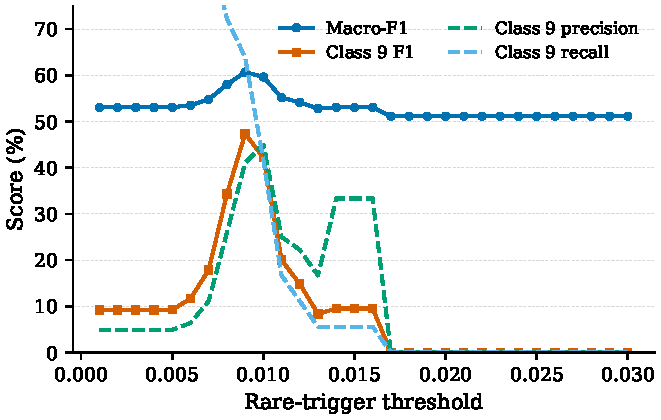
\includegraphics[width=0.65\linewidth]{figures/fig6_threshold_sensitivity.pdf}
  \caption{Rare-trigger threshold sensitivity. A low threshold is needed for rare-fault recall; too aggressive triggering reduces precision. The calibrated threshold (dashed line) is near the optimal region.}
  \label{fig:threshold}
\end{figure}
